% !TEX root = MAIN.tex

\subsubsection{KLEE}

\INDEX{KLEE}~\cite{cadar2008klee} is an open source tool that implements {\INDEX{Concolic Execution}}, a technique that performs \INDEX{symbolic execution} along a concrete execution path. KLEE was designed to automatically generate test cases that achieve high code coverage. The tool is implemented as a modified LLVM virtual machine that targets LLVM bytecode programs.
KLEE also provides a symbolic POSIX library that enable analysis of programs that uses the system's environment. For example, KLEE can be executed with the flag \texttt{-sym-stdin N} which will make stdin symbolic with size \texttt{N}.  

In the context of FAQAS, we aim to rely on KLEE to automatically produce the inputs that make the mutated version of the program generate a different output than the original version.
This is observed in the outcome of the verification being \emph{true}, i.e., the assertion indicating that the output of the original and mutated program are different does hold. In this case, KLEE produces the values of the inputs for which both versions of the program have a different result.

When the outcome of the verification is \emph{false}, the assertion that indicates if the output of the original and mutated program are the same does not hold. A \emph{false} outcome means that the mutant is equivalent and thus the test case can be ignored. 
We only consider the test inputs produced when the verification of the assertion holds.

% !TEX root =  ../MAIN.tex
\begin{minipage}{14cm}
\begin{lstlisting}[style=CStyle, caption=Example of code for the identification of inputs with KLEE., label=GSLaugmentation_klee]
/* Copyright (c) 2013-2017 GomSpace A/S. All rights reserved. */
  
#include <gs/util/byteorder.h>
#include <assert.h>

...

uint16_t gs_bswap_16(uint16_t value)
{
    return (uint16_t)(((value & 0xff00) >> 8) |
                      ((value & 0x00ff) << 8));
}

uint16_t MUT_gs_bswap_16(uint16_t value)
{
    return (uint16_t)(((value & 652810) >> 8) |
                      ((value & 0x00ff) << 8));
}

...

int main()
{
    uint16_t valueSymbolic;
    klee_make_symbolic(&valueSymbolic, sizeof(valueSymbolic), "valueSymbolic");

    uint16_t res = gs_bswap_16(valueSymbolic);
    uint16_t resMUT = MUT_gs_bswap_16(valueSymbolic);

    assert(res != resMUT);
    
    printf ("res %u resMUT %u\n", res, resMUT);
} 
\end{lstlisting}
\end{minipage}


Listing~\ref{GSLaugmentation_klee} shows an example of generation of inputs with KLEE for the mutant \linebreak\emph{MUT\_gs\_bswap\_16} presented in Listing~\ref{GSLaugmentation}. In this case, the function \emph{main} is used to declare all the variables and assertions to be processed by KLEE to generate the required inputs for testing. Particularly, the function creates an input of type \texttt{uint16\_t} with a symbolic value given by the KLEE function \texttt{klee\_make\_symbolic}. The symbolic value is then passed to both the original and the mutated functions. To produce test inputs that kill mutants the assertion of Line 30 should be inserted.

To run this example, the program must be compiled with clang, instead of its original compiler, and with the \texttt{-emit-llvm} option enabled, since KLEE runs on bitcode rather than source code or binaries. The command used to compile this example is the following:

\begin{verbatim}
clang -DKLEE -I ~/klee/include -Iinclude -emit-llvm -c -g -O0 -Xclang 
-disable-O0-optnone byteorder.c
\end{verbatim}

By default, KLEE works on programs that do not use any external code such as C library functions. To enable KLEE to work with external code, the KLEE POSIX runtime capability should be enabled. To generate the test inputs for this example, the following command should be used:

\begin{verbatim}
~/klee/build/bin/klee --libc=uclibc --posix-runtime byteorder.bc
\end{verbatim}



\begin{figure}[h]
\begin{center}
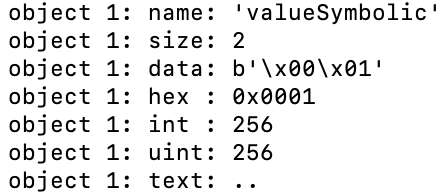
\includegraphics[width=0.4\textwidth]{images/klee_output_1}
\caption{KLEE output}
\label{fig:klee_output_1}
\end{center}
\end{figure}

% !TEX root =  ../MAIN.tex
\begin{minipage}{14cm}
\begin{lstlisting}[style=CStyle, caption=Example of test case for function \emph{gs\_bswap\_16} derived from KLEE output., label=GSLaugmentationTest_klee]
int main(){
    uint16_t v = 256;                                                                                                                                  
    uint16_t res;
    uint16_t resMUT;

    res = gs_bswap_16(v);
    resMUT = MUT_gs_bswap_16(v);

    assert( res == resMUT );
    return 0;
}
\end{lstlisting}
\end{minipage}


Figure~\ref{fig:klee_output_1} shows the output generated by KLEE when processing the function. It indicates that for the input \emph{symbolicValue=256}, the outcome of the assertion \texttt{res != resMUT} holds. Listing~\ref{GSLaugmentationTest_klee} shows a test case manually written based on the output produced by KLEE.

% !TEX root =  ../MAIN.tex

\begin{lstlisting}[style=CStyle, caption=Second example of code for the identification of inputs with KLEE., label=GSLaugmentationTwo_klee]
#include <klee/klee.h>

#include <gs/util/base16.h>
#include <stdio.h>
#include <stdlib.h>
#include <limits.h>
#include <ctype.h>
#include <errno.h>
#include <assert.h>


int base16_decode(const char *encoded, uint8_t *raw)
{
    uint8_t *raw_bytes = raw;
    if (encoded) {
        const char *encoded_bytes = encoded;
        char buf[3];
        char *endp;

    while (encoded_bytes[0]) {
            if (!encoded_bytes[1]) {
                return GS_ERROR_ARG;
            }
            memcpy(buf, encoded_bytes, 2);
            buf[2] = '\0';
            *(raw_bytes++) = (uint8_t) strtoul(buf, &endp, 16);
            if (*endp != '\0') {
                return GS_ERROR_ARG;
            }
            encoded_bytes += 2;
    }
    }
    return (int)(raw_bytes - raw);
}

int MUT_base16_decode(const char *encoded, uint8_t *raw)
{
    uint8_t *raw_bytes = raw;
    if (encoded) {
        const char *encoded_bytes = encoded;
        char buf[3];
        char *endp;

    while (encoded_bytes[0]) {
            if (!encoded_bytes[1]) {
                //return GS_ERROR_ARG;
            }
            memcpy(buf, encoded_bytes, 2);
            buf[2] = '\0';
            *(raw_bytes++) = (uint8_t) strtoul(buf, &endp, 16);
            if (*endp != '\0') {
                return GS_ERROR_ARG;
            }
            encoded_bytes += 2;
    }
    }
    return (int)(raw_bytes - raw);
}


#ifdef KLEE
int main() 
{
    char encoded[4];
    char a,b,c;
    klee_make_symbolic(&a, sizeof(a), "a");
    klee_make_symbolic(&b, sizeof(b), "b");
    klee_make_symbolic(&c, sizeof(c), "c");
    uint8_t raw;
    uint8_t mRaw;
    int ret;
    int mret;

    
    encoded[0]=a;
    encoded[1]=b;
    encoded[2]=c;
    encoded[3]=0;

    raw=0;
    ret = base16_decode(encoded,&raw);

    encoded[0]=a;
    encoded[1]=b;
    encoded[2]=c;
    encoded[3]=0;

    mRaw=0;
    mret = MUT_base16_decode(encoded,&mRaw);
    printf ("ret %d mret %d\n", ret, mret);

    assert( ret != mret );
} 
#endif
\end{lstlisting}
\begin{lstlisting}[style=CStyle, caption=Test case derived for the example in Listing~\ref{GSLaugmentationTwo_klee}., label=GSLaugmentationTwo_kleeTest]
int main(){
    char encoded[4];

    uint8_t raw;
    int ret;

    encoded[0]=48;
    encoded[1]=0;
    encoded[2]=0;
    encoded[3]=0;

    raw=0;
    ret = base16_decode(encoded,&raw);


    assert( ret == GS_ERROR_ARG );
    return 0;
}
\end{lstlisting}



Listing~\ref{GSLaugmentationTwo_klee} shows another example of a source file to be parsed by KLEE to automatically derive inputs for a test case. 

Similar to Section~\ref{subsec:cbmc}, we also apply KLEE to the mutant \texttt{MUT\_base16\_decode}. Function \emph{main} provide the setup for KLEE. In this case, similarly to the case of CBMC, we specify that we expect \texttt{ret == mret} by writing \texttt{klee\_assume(ret == mret)}. In this case the test case can be generated by running

\begin{verbatim}
~/klee/build/bin/klee --libc=uclibc --posix-runtime 
-silent-klee-assume byteorder.bc
\end{verbatim}

\CHANGED{The main difference with respect to the command used for Listing~\ref{GSLaugmentation_klee} is  that the command above identifies only the inputs that invalidate the assertion (i.e., the set of klee outputs is reduced). The set of inputs generated by KLEE can be further reduced to one by adding \texttt{klee\_silent\_exit(0);} after the call to \texttt{klee\_assume}. In FAQAS, we plan to rely on this configuration.}

Function \emph{main} in Listing~\ref{GSLaugmentationTwo_kleeTest} is the test case manually derived from the KLEE output.

Comparing Listings~\ref{GSLaugmentationTwo} and~\ref{GSLaugmentationTwo_klee} can be seen the advantages of KLEE over CBMC; basically, is it no longer necessary to provide the implementation of standard library functions (e.g., \emph{strtoul}), because they are provided by the POSIX runtime capability. This capability makes easier the integration of KLEE with the case study systems of FAQAS, and makes the results more accurate, since KLEE is aware of the standard library functions definitions and implementations. One of the disadvantages of KLEE is that it relies on CLANG/LLVM which may prevent the possibility to apply it to source files containing architecture-specific instructions not supported by LLVM (see Section~\ref{subsec:mull}). However, there is no guarantee that CBMC can correctly process source files that cannot be processed by LLVM.

